\documentclass[10pt,a4paper]{article}
\usepackage[latin1]{inputenc}
\usepackage[margin=1in]{geometry}
\usepackage{amsmath}
\usepackage{amsfonts}
\usepackage{amssymb}
\usepackage{graphicx}
\begin{document}
	
\section{Tower Lift System}

\begin{figure}[h!]
	\centering
	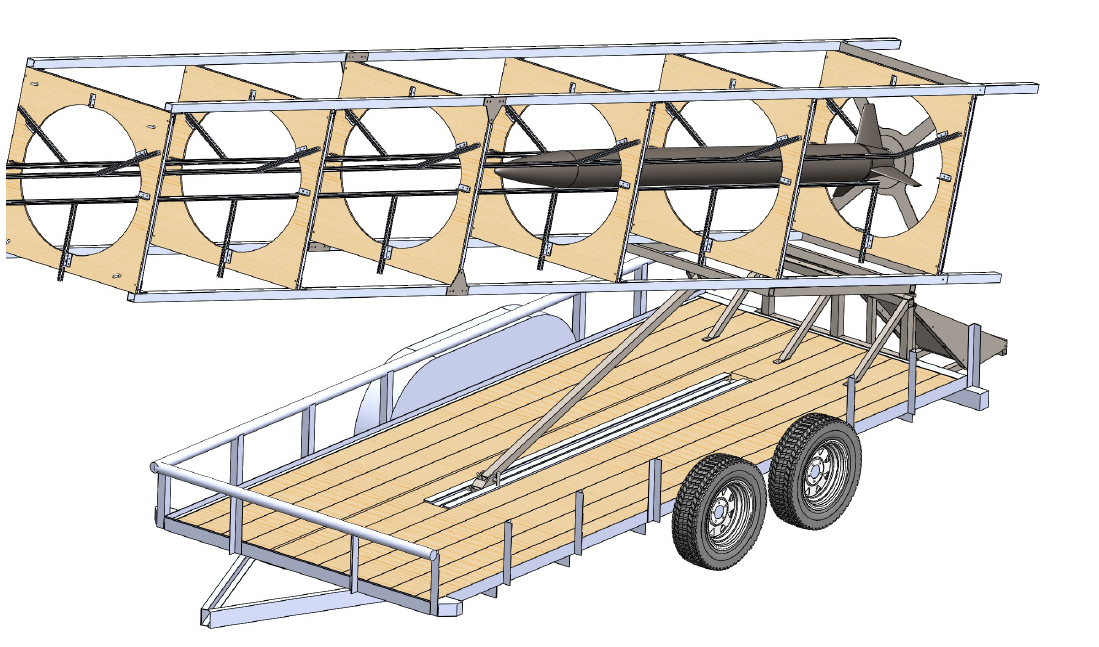
\includegraphics[width=0.75\textwidth]{./figs/Overview.png}
	\caption{Lift System Overview}
	\label{fig:overview}
\end{figure}


\begin{table}[h!]
		\centering
		\begin{tabular}{l l l}
			Component & Major Dimensions & Weight \\
			A36 Steel Flanges(2) & 3in x 6in x 3/8in  & NEEDNAME \\
			A36 Steel Sled with 6 extruded 5/8" holes & 1in x 6in x 3in & NEEDNAME \\
			A36 Steel Vertical Support & 1/8in x 2in x 3in & NEEDNAME\\
			A36 Steel Association I-beam (2) & 3in x 2.5in x 101in & NEEDNAME\\
			A36 Steel Clevis & 6.25in x 2.5in x 2in & NEEDNAME\\
			A36 Square Tubing & 2in x 2in x 82in & NEEDNAME\\
			PCI-PTR-1.50 Track Rollers (6) & 1.5in x 2.69in x 5/8in dia & NEEDNAME\\
			Superwinch 12 volt DC powered Electric Winch & 21in x 6.5in x 8 3/4in & 50lb \\
			
			
		\end{tabular}
		\caption{Subsystem Specifications}
		\label{tab:example}
\end{table}


\subsection{Design}

	The lift system is semi-automated, winch powered mechanism made to raise the launch tower. The primary function of this lift is to provide a stable operating system for erecting the tower from the launch trailer. This system streamlines the process of setting up the tower by decreasing the amount of time and human power required. additionally, the lift is designed ot accommodate varying rocket weights and multiple loads. \\
	
\subsubsection{Requirements}
The lift system will need to meet these engineering specification:
\begin{itemize}
	\item Be mobile and robust
	\item Raise and lower the tower
	\item Attach to the steel frame support
\end{itemize}

\subsubsection{Solutions}
	The lift system will consist of four major components; a track, a sled, clevis, and a lever arm. The steel track is bolted onto the frame of the launch trailer which will restrict the movement of the sled to horizontal translation. The sled is a solid steel block with 6 heavy duty track rollers designed to withstand heavy loads with two welded flanges. Also, the sled is coupled with a winch line that will enable the sled to move along the track. The two flanges on the sled and the clevis are connected to a square tube lever arm by a prefabricated hitch pins. The clevis comprised of two flanges with a 90 degree cut at the base and welded onto the launch tower support.\\
\subsubsection{Track}
In order to insure a straight path for the sled to travel along, two A36 steel I-beams are placed down the middle of the trailer. The lips that flank either side of the vertical member of the used at the support for the beam off a place for the rollers to travel and bear the force applied during the lifting process. During the lifting process, the rails will be exposed to the moments caused by the weight of the tower and rocket.Refer to Figure  \ref{fig:Calculation of Moments}\\

\begin{figure}
\centering
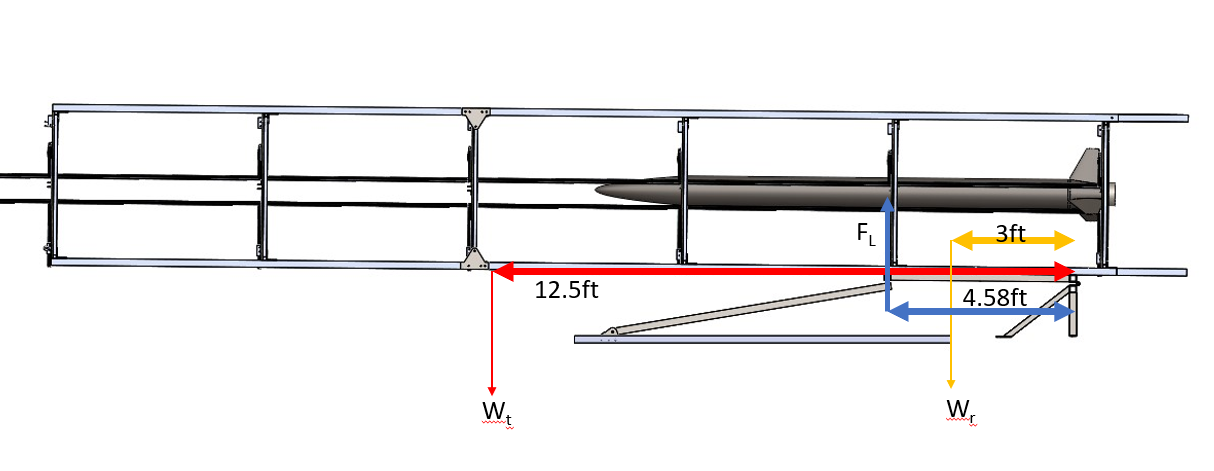
\includegraphics[width=0.75\textwidth]{./figs/moment_cal.png}
\caption{Calculation of Moments}
\label{fig:Calculation of Moments}
\end{figure}

\begin{equation}
\sum(M_{o}) = W_{t}*12.5ft+ W_{r}*3ft -F_{L}*4.58ft=0 
\end{equation} 
\label{eq:1}\\
Substituting in the known variables $[W_t , W_r]$  and solving for $[F_L]$ produces a force of $897.92$ $lb_f$
Which is within the yield values of the I-Beams. Furthermore, to prohibit any unwanted degrees of freedom the I-Beams are spaced exactly 7.5in  apart while leaving a space of 1/8in from the edge of the roller to the vertical face of the I-beam.Also, to accurately place the beams with the previously stated spacing, the track is bolt on to the frame of the trailer by 6 3/8in by 1in hardware.


\subsubsection{Rollers}
 The specifications constraints attributed from the reactionary forces during the power lift narrowed down the mechanism used for translational movement. Additionally, a short degree of travel and distance needed eliminated any prefabricated methods such as hydraulics. Researching further into the movement of systems under heavy load, rollers made specifically for travel along tracks became the front runner offering both simplicity and robustness. PCI, Procal inc. manufactures rollers with multiple applications and will assure certified load carrying rollers. PCI-PTR- 1.5in x 2.69in track rollers was selected due to the short axle length and properties under load. 
 \subsubsection{Sled}
 The sled will bear and exert a force during the entirety of the lift and lowering of the trailer. In figure \ref{fig:forces} calculations at the beginning angle and the force needed to lift the launch tower were implemented to find the overall max force experienced. Using the force in the y-direction computed in equation \eqref{eq:1} the overall force $(F_o)$ is equal to 5110.23 $lb_f$ eqn. \ref{eq:4} with a component in the x-direction $(f_x)$ of 5030.5 $lb_f$ eq.\ref{eq:3}. Due to the these loads, A36 steel was chosen due to its yield properties. Two 3/8in flanges will have a hitch pin connection to either side of the lever arm in order to uniformly distribute the force throughout the sled.  
\begin{figure}
	\centering
	\includegraphics[width=0.75\textwidth]{./figs/forces.png}
	\caption{Calculation of Tri-Directional Forces}
	\label{fig:forces}
\end{figure}
\begin{equation}
10.12^o = \tan(\frac{F_y}{F_x})
\end{equation} 

\begin{equation}
F_x = \frac{897.92lb_f}{\arctan{10.12}}
\end{equation}
\label{eq:3}
\begin{equation}
\sin(10.12) = \frac{897.92}{F_o}
\end{equation}
\label{eq:4}



\subsection{Lever Arm}
The lever arm of the lift is a 82in long, 2in square A36 steel beam. Buckling analysis was preformed on the lever arm in order to minimize the risk of failure. NEED TO TALK TO AARON ABOUT CAL. \\

Due to the $\frac{L}{K}_{actual}$ is less than the $\frac{L}{K}_ {critical}$ the Johnson equation can be applied.  \\


\begin{equation}
\frac{L}{K}_actual = \frac{L}{\sqrt{I/A}}
\end{equation}
\begin{equation}
\frac{L}{K}_{actual} = \frac{79.6}{\sqrt{.07523/2^2-1.625^2}} = 107.0
\end{equation}
\begin{equation}
\frac{L}{K}_ {critical} =\sqrt{\frac{\pi^2*E}{\frac{S_y}{2}}} = 126.1
\end{equation}


Due to the $\frac{L}{K}_{actual}$ is less than the $\frac{L}{K}_ {critical}$ the Johnson equation can be applied.  \\

\begin{equation}
\frac{P_{cr}}{A} = S_{yc} - \frac{1}{E} * (\frac{S_{yc} * (\frac{L}{K})}{2*pi}^2)
\end{equation}
\begin{equation}
{P_{cr}} = 36ksi - \frac{1}{29,000ksi} * (\frac{36ksi(107)}{2*pi})^2 *({2^2-1.625^2})
\end{equation}
Once the force critical ($P_cr$) the ratio of force critical and force actually applied can be used to solve for the safety factor of the lever arm.   \\
\begin{equation}
n_{saftey factor} = \frac{P_{cr}}{P_{actual}}
\end{equation}
\begin{equation}
	n_{saftey factor} = \frac{31,300}{5110} = 6.13
\end{equation}
A safety factor of 6.13 states the lever arm can with endure more than six times the load being applied to it during the lifting process. 

\subsubsection{Clevis}
The steel frame on the launch tower is constructed out of A36 steel 2in square tubing which creates a platform for integrating a clevis. The angle created by the lever arm will transition from 10.15 to a final angle of 60 caused a constraint with the placement of the clevis. A clevis mounted parallel from a face of the support frame would cause a torsion to occur in the steel horizontal support. \\

\begin{figure}
	\centering
	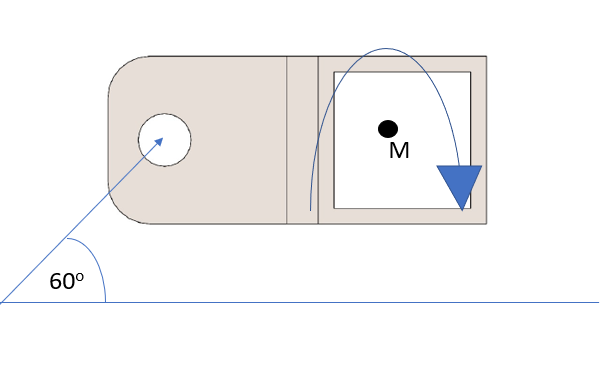
\includegraphics[width=0.75\textwidth]{./figs/clevis_angle_60.png}
	\caption{Moment at the Support at 60 degrees}
	\label{fig:angle_60}
\end{figure}

Further design changes led to Two 1in flanges are welded into place at a 45 degree angle and allot for a pin connection to the lever arm. Additionally, as the tower is being raised, the load transfers from the lever arm to the hinge located on the trailer. \ref{fig:load_graph} \\
\begin{figure}
	\centering
	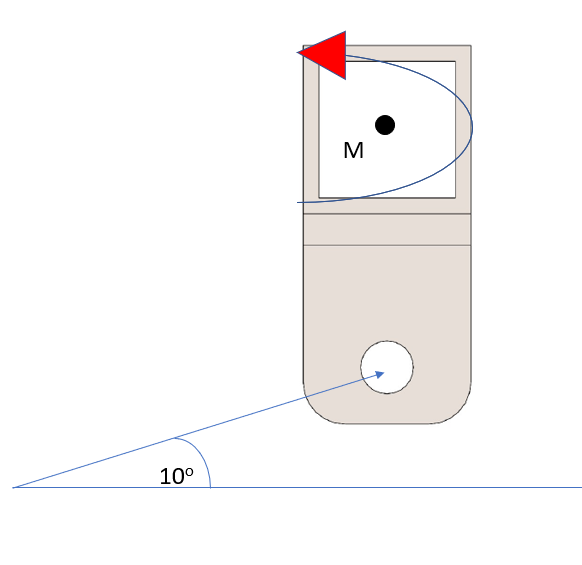
\includegraphics[width=0.75\textwidth]{./figs/clevis_angle_10.png}
	\caption{Moment at the Support at 10 degrees}
	\label{fig:angle_10}
\end{figure}
\begin{figure}
		\centering
		\includegraphics[width=0.75\textwidth]{./figs/load_graph.png}
		\caption{Load transferring as the tower is raised}
		\label{fig:load_graph}
\end{figure}

 
\begin{figure}
	\centering
	\includegraphics[width=0.75\textwidth]{./figs/clevis_good_10.png}
	\caption{Moment at the Support at 10 degrees}
	\label{fig:angle_10}
\end{figure} 
\subsubsection{Winch}
A winch is used for horizontal pulling and present a reliable source of power. Due to the ability to extract and retract under load, the Super-winch Tiger winch with a max load of 10,000 $lb_f$ was chosen. The winch is integrated to the launch trailer by adapting cradle to be welded on to the frame of the trailer. 

\subsection{Manufacturing}
The malleability of A36 steel leads to many options in the manufacturing process. The tracks, rollers, and lever arm were ordered to meet our specifications. The sled is cut from a larger stock of 2 in thick steel, then drilled a 3/8in hole for the pin connection. The 3/8in thick flanges are cut out using a laser cutter for precision. The sled and two flanges are then welded together on either side with the addition of a vertical support member. \\
The clevis flanges are cut using INSERT MANUFACTURING HERE

 
\subsection{Testing}
N/A\\


\begin{thebibliography}{10}
	
	\bibitem{example}
	Fernandez, M.M., 
	"Propellent Tank Pressurization Modeling for a Hybrid Rocket,"
	Thesis, Mechanical Engineering Dept., Rochester Institute of      
	Technology, 
	Rochester, NY, 2009.
	
\end{thebibliography}

\end{document}